% % % Uncomment the Preamble, titles and begin/end document  % % %
% % % AND comment the input line in the main document (thesis) to run solo % % %


%\documentclass{article}

%\usepackage{setspace}
%\usepackage{epsfig}  % for figures
%\usepackage{graphicx}  % another package that works for figures
%\usepackage{subcaption}  % for subfigures
%	\captionsetup{subrefformat=parens} %automatic parentheses around subrefs
%\usepackage[font = small]{caption}
%\usepackage{amsmath}  % for math spacing
%\usepackage{amssymb}  % for math spacing
%\usepackage{url}  % Hyphenation of URLs.
%\usepackage{lscape}  % Useful for wide tables or figures.
%\usepackage{times}  %change font to times new roman!! take that computer modern!
%\usepackage{pgfgantt}
%\usepackage[margin=1in]{geometry}

%\title{Results for Low Incidence Infection}

%\begin{document}
%\maketitle

\section{Results for Low Incidence Infection}

The effects of a small, low density infection within a nematode population were evaluated. Unique combinations of virus characteristics including infection rates, virulences, and viral loads were tested \ref{tbl:lowiiprops}.  The simulation was performed over 5 iterations per treatments over 5 years with data recorded at 4 day intervals.  Additionally, the simulation was repeated 20 times for a total of 100 replicates per unique combination.  The environment agent was set to temperature data from Champaign County, IL.    (Nematode settings and crops planting every year)  

% TABLE - Initial conditions
\begin{table}[htpb]
\caption[Low Incidence Infection Parameters]{Simulation parameters for the low incidence infection treatment.}
\centering
\label{tbl:lowiiprops}
\begin{tabular}{|c r r p{3in}|}
	\hline
		Agent & Variable & Value(s) & Units \\
	\hline
		Virus &          &          &  (what are some of these units?)     \\
		      & Durability & $0.2$ &\\
		      & Viral Loads & $0.1, 0.2, 0.5, 1, 2, 5, 10$ & Rate of health depletion\\
		      & Infection Rate & $0, 0.01, 0.1, 0.2, 0.5$ & Initial proportion of population infected \\
		      & Transmissbility & $0.5$    &  The contagiousness of an infected SCN.  The probability of an infection SCN to spread the virus to a healthy SCN. \\ 
		      & Virulence & $ 0.2,0.8, 1, 1.2$    &    \\
	\hline
\end{tabular}
\end{table}

\section{Objectives}
\begin{enumerate}
\item Determine how the low incidence infections affect the Nematode populations over time
\item Determine how similar/ different varying levels of infection rates affect the various life stages of the SCN
\item Determine which parameters are responsible for resulting changes in nematode populations
\end{enumerate}

\section{Results and Discussion}


\subsection{Distribution analysis--Kolmogrov Smirnov}

To visually discern whether or not the virus infection had an impact on SCN populations over time, the nematode population data were compared between the low incidence infection treatments and the zero infection treatments using the Kolmogrov-Smirnov (KS) test.  

% %  Kolmogrov-Smirnov Figures
\begin{figure}[ht]
	\centering
		
		
	\begin{subfigure}[b]{0.45\textwidth}{
		\includegraphics[width = \linewidth]{../Analysis/lowinf-zeroinf/figs/Virulence_ks_lowii.pdf}
		%\enskip %horizontal spacing
		\subcaption[D stat Across Virulences]{Virulences}
		\label{fig:ks_Vir}  %label MUST go after caption
		}
	\end{subfigure}
~  %space between figures
	\begin{subfigure}[b]{0.45\textwidth}{
		\includegraphics[width = \linewidth]{../Analysis/lowinf-zeroinf/figs/Infrate_ks_lowii.pdf} 
		\subcaption[D stat Across Infection Rates]{Infection Rates}
		\label{fig:ks_InfR}
		}
	\end{subfigure}
	
	\begin{subfigure}[b]{0.8\textwidth}{
		\centering
		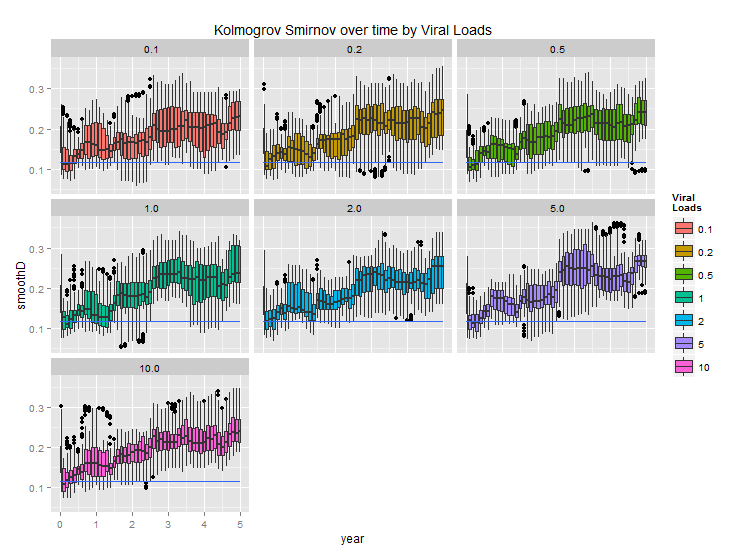
\includegraphics[width =\linewidth]{../Analysis/lowinf-zeroinf/figs/VLoad_ks_lowii.pdf}
		\subcaption[D stat Across Viral Loads]{Viral Load}
		\label{fig:ks_VLoad}
		}
	\end{subfigure}

\caption[Kolmogrov-Smirnov evaluation of Nematode Populations over Time]{The D stat was calculated between infected and non-infected SCN populations and evaluated over time across initial virulences \subref{fig:ks_Vir}, infection rates \protect\subref{fig:ks_InfR}, and viral loads \protect\subref{fig:ks_VLoad}. All boxplots have a width of 0.1 years.  Baselines are drawn in each plot, which were derived from Kolmogrov-Smirnov statistics calculated between randomized subsamples of SCN populations within the low incidence infection treatment, to compare the results with natural variation of the D statistic.}
\end{figure}


\subsection{Virus Parameters over Time}
	Viral virulences decreased over time with respect to initial infection rates in all cases. These decreases were each significantly different from the control treatment ($p < 0.0001$, Kruskal-Wallis Test). Furthermore, it appeared the infection rates that were tested significantly affected the distributions of virulence values over time. (maybe we should do nested hypothesis testing?  test the virulences at certain years against other years and then across infection rates?)    

\begin{figure}[htpb]
	\centering
	\includegraphics
		[width = \linewidth]{../Analysis/lowinf-zeroinf/figs/logVir_time_overInfRates.pdf}
	\caption[Effect of Infection Rates on Virulence over Time]{blah}
	\label{fig:logVir_IR}
\end{figure}

\subsection{Contributing factors to Nematode Suppression}

\begin{table}[htpb]
\caption[Mean Nematode Populations Across Infection Rates]{Reported nematode means after 5 years.  The Wilcoxon Rank Sum test was used to determine the significance of infection. Standard Deviations are in parentheses (n = 50 for control, n = 100 for the rest)}
\centering
\label{tbl:infR_stat}
\begin{tabular}{c r r r r r r}
	\hline
		 Crop Year & 0 & 1 &  2 & 3 & 4 & 5\\
	\hline
	    Infection Rate & & & & & & \\
	\hline
		0              & 9334     & 14857    &  24647   & 34552    &  &  \\
		0.01 & &      & Durability & $0.2$ && \\
		0.1  & &      & Viral Loads & $0.1, 0.2, 0.5, 1, 2, 5, 10$ && \\
		0.2  & &      & Infection Rate & $0.01, 0.1, 0.2, 0.5$ & & \\
		0.5  & &      & Transmissbility & $0.5$    &&      \\
	\hline
\end{tabular}
\end{table}

\begin{figure}[htpb]
	\centering
	\includegraphics
		[width = \linewidth]{../Analysis/lowinf-zeroinf/figs/Nemxyear_subdensityplot.pdf}
	\caption[Effect of Infection Rates on Nematode Population Over Time ]{Effect of Infection Rates on Nematode Population Over Time }
	\label{fig:Nemsub_Vir}
\end{figure}











%\end{document}

